
\chapter{ Chapter Title } \label{chapter-fml}

% --------
\minitoc
% --------

In general ...

\newpage

The value ... 

\vskip0.1in

\begin{itemize}
    \item \textbf{Timestamp}: The date and time for each interval.
    \item \textit{Timestamp}: The date and time for each interval.
    \item \underline{Timestamp}: The date and time for each interval.
\end{itemize}

% ------------------------------------------------------------ -- %
\section{ section 1}
% ------------------------------------------------------------ -- %

Let $V_{t}$.

\vskip0.1in

% ********************************************************* PLOT **
\begin{figure}
    \centering
    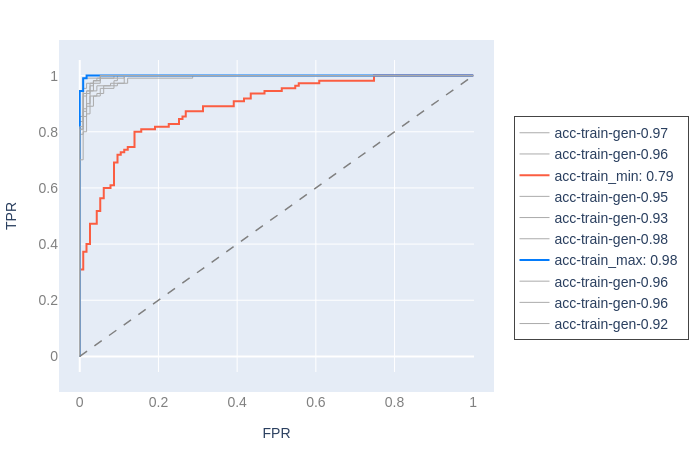
\includegraphics[width=9cm, height=5cm, keepaspectratio=false]{figures/plot-rocs.png}
    \caption{\footnotesize \textit{Subtext for the plot}}
    \label{fig-ohlcprices}
\end{figure}
% *****************************************************************

\autoref{fig-ohlcprices}